	%===================================================================================
% JORNADA CIENTÍFICA ESTUDIANTIL - MATCOM, UH
%===================================================================================
% Esta plantilla ha sido diseñada para ser usada en los artículos de la
% Jornada Científica Estudiantil, MatCom.
%
% Por favor, siga las instrucciones de esta plantilla y rellene en las secciones
% correspondientes.
%
% NOTA: Necesitará el archivo 'jcematcom.sty' en la misma carpeta donde esté este
%       archivo para poder utilizar esta plantila.
%===================================================================================



%===================================================================================
% PREÁMBULO
%-----------------------------------------------------------------------------------
\documentclass[a4paper,10pt,twocolumn]{article}

%===================================================================================
% Paquetes
%-----------------------------------------------------------------------------------
\usepackage{amsmath}
\usepackage{wrapfig}
\usepackage{amsfonts}
\usepackage{amssymb}
\usepackage{jcematcom}
\usepackage{algorithm}
\usepackage{algorithmic}
\usepackage[utf8]{inputenc}
\usepackage{listings}
\usepackage{color}
\usepackage{graphicx}
\usepackage[pdftex]{hyperref}
\usepackage{tikz}
%-----------------------------------------------------------------------------------
% Configuración
%-----------------------------------------------------------------------------------
\hypersetup{colorlinks,%
	    citecolor=black,%
	    filecolor=black,%
	    linkcolor=black,%
	    urlcolor=blue}

%===================================================================================
\lstset{frame=tb,
	language=python,
	aboveskip=3mm,
	belowskip=3mm,
	showstringspaces=false,
	columns=flexible,
	basicstyle={\small\ttfamily},
	numbers=none,
	numberstyle=\tiny\color{gray},
	commentstyle=\color{dkgreen},
	breaklines=true,
	breakatwhitespace=true,
	tabsize=3
}



%===================================================================================
% Presentacion
%-----------------------------------------------------------------------------------
% Título
%-----------------------------------------------------------------------------------
\title{Compilador para lenguaje COOL}

%-----------------------------------------------------------------------------------
% Autores
%-----------------------------------------------------------------------------------
\author{\\
\name Isabella Sierra \email \href{mailto:isabellamaria.sierra@estudiantes.matcom.uh.cu}{isabellamaria.sierra@estudiantes.matcom.uh.cu}
	\\ \addr Grupo C412 \AND
\name Adrian Tubal Páez Ruiz \email \href{mailto:a.paez@estudiantes.matcom.uh.cu}{a.paez@estudiantes.matcom.uh.cu}
	\\ \addr Grupo C412  \AND
\name Eric Martín García \email \href{mailto:e.martin@estudiantes.matcom.uh.cu}{e.martin@estudiantes.matcom.uh.cu}
	\\ \addr Grupo C411 
 }

%-----------------------------------------------------------------------------------
% Tutores
%-----------------------------------------------------------------------------------
\tutors{\\
	Alejandro Piad, \emph{Universidad de La Habana}}
%-----------------------------------------------------------------------------------
% Headings
%-----------------------------------------------------------------------------------
%\jcematcomheading{\the\year}{1-\pageref{end}}{A. Páez, I. Sierra, M. Perdomo}

%-----------------------------------------------------------------------------------
\ShortHeadings{Compilador para lenguaje COOL}{Autores}
%===================================================================================



%===================================================================================
% DOCUMENTO
%-----------------------------------------------------------------------------------
\begin{document}

%-----------------------------------------------------------------------------------
% NO BORRAR ESTA LINEA!
%-----------------------------------------------------------------------------------
\twocolumn[
%-----------------------------------------------------------------------------------

\maketitle

%===================================================================================
% Resumen y Abstract
%-----------------------------------------------------------------------------------
\selectlanguage{spanish} % Para producir el documento en Español

%-----------------------------------------------------------------------------------
% NO BORRAR ESTAS LINEAS!
%-----------------------------------------------------------------------------------
\vspace{0.8cm}
]
%-----------------------------------------------------------------------------------


%===================================================================================

%===================================================================================
% Introducción
%-----------------------------------------------------------------------------------
%===================================================================================



%===================================================================================
% Desarrollo
%-----------------------------------------------------------------------------------
\section{Lexer y Parser}

Para resolver la sintáctica del compilador se utilizó el módulo de Python \textbf{PLY} que implementa las populares herramientas de construcción de compiladores \textit{lex} y \textit{yacc}, generando el primer \textbf{AST} del proceso de compilación.

\subsection{Tokenización con lex}

\begin{enumerate}
	\item Creación de los tokens: 
	Una instancia de objeto \textbf{LexToken} (llamemos a este objeto \textbf{t} ) tiene los siguientes atributos:
	\begin{itemize}
		\item \textbf{t.type} que es el tipo de token (por ejemplo: 'INT' , 'PLUS' , etc.).
		\item \textbf{t.value} que es el lexema
		\item \textbf{t.lineno} que es el número de línea actual
	\end{itemize} 

	\item Creación de las reglas: Las reglas de expresiones regulares pueden definirse como un \textbf{string} o como una función. En cualquier caso, el nombre de la variable tiene el prefijo \textbf{t\_} para denotar que es una regla para hacer coincidir tokens.
	
	Para tokens simples, la expresión regular se especificó como \textbf{string}: $t\_PLUS = r'\backslash+'$
	
	Para tokens mas complejos se definieron funciones:
	
	\begin{algorithm}
		\caption{Ejemplo 1}
		\begin{algorithmic}
			\STATE def t\_STRING(t):
			\STATE $\;\;\; $ r'""'
			\STATE $\;\;\; $ t.lexer.string\_start = t.lexer.lexpos
			\STATE $\;\;\; $ t.lexer.begin('string')
		\end{algorithmic}
	\end{algorithm}
	\item Creacion del lexer: $ lexer = lex.lex()$
\end{enumerate}

\subsection{Parsing con yacc}

Una vez terminado el proceso de tokenización se realiza el proceso de parsing utilizando la herramienta \textit{yacc}. Luego de la creación de una gramática libre del contexto \textit{yacc} generará un parser \textbf{LALR}.\\

Cada regla de la gramática será definida por una función donde el \textbf{string} de documentación de esa función contiene la especificación apropiada. Las declaraciones que conforman el cuerpo de la función implementan las acciones semánticas de la regla junto con las definiciones de los nodos del \textbf{AST}.

\begin{algorithm}
	\caption{Ejemplo 2}
	\begin{algorithmic}
		\STATE def p\_atom\_atring(p):
		\STATE $\;\;\; $ '''atom : STRING'''
		\STATE $\;\;\; $ p[0].add\_location(p.lineno(1)),
		\STATE $\;\;\; $ p[0] = StringNode(p[1])
		\STATE $\;\;\; $ find\_column(p.lexer.lexdata, p.lexpos(1)))
	\end{algorithmic}
\end{algorithm}

Al finalizar el proceso de parsing, estarán todas las condiciones creadas para iniciar el chequeo semántico.

\section{Chequeo semántico}

Para realizar el chequeo semántico se utilizó un \lstinline|visitor| de una pasada que realiza las siguientes acciones sobre un nodo:

\begin{itemize}
	\item Aplica el \lstinline|visitor| correspondiente a las expresiones hijas involucradas y de éste se obtiene el tipo estático inferido de cada una. 
	\item Se aplican las reglas de chequeo de tipos definidas para cada una de las operaciones para detectar errores. 
	\item Se infiere el tipo estático de la expresión representada por el nodo y se retorna para ser utilizado por sus padres. 
\end{itemize}

\subsection{CoolType}
Para auxiliarnos en el chequeo semántico definimos una clase \lstinline|CoolType| que envuelve la significancia de un tipo en \textit{COOL}. 

Contiene los atributos:

\begin{itemize}
	\item \lstinline|name|: Representa el nombre del tipo. 
	\item \lstinline|inherits|: Determina si la clase es heredera de alguna clase definida en el programa. 
	\item \lstinline|parent|: Es una instancia \lstinline|CoolType| que representa el padre de la clase definida. 
	\item \lstinline|methods|: Contiene todos los métodos definidos por la clase (De tipo \lstinline|CoolTypeMethod|). 
	\item \lstinline|attributes|: Contiene los atributos definidos por la clase (De tipo \lstinline|CoolTypeAttribute|).
	\item \lstinline|childs|: Contiene todas los \lstinline|CoolType| que heredan directamente de la clase. 
	\item \lstinline|order_interval|: Atributo que define un intervalo $(x, y)$ tal que si $A\leq B$, entonces $(x_A, y_A)$ estará contenido en $(x_B, y_B)$. Más adelante explicaremos para qué se utiliza este atributo. 
\end{itemize}

y los métodos: 

\begin{itemize}
	\item \lstinline|get_method|: Obtiene el método determinado por el argumento \lstinline|id|, teniendo en cuenta si pudo haber sido definido por la clase guardada en \lstinline|parent|. 
	\item \lstinline|get_all_methods|: Obtiene todos los métodos definidos por la clase, así como los definidos por alguna clase superior en su línea de herencia. 
	\item \lstinline|add_method|: Agrega el método con nombre \lstinline|id| en el conjunto de métodos de la clase. Esta función tiene implícitas las reglas de definición de métodos. 
	
	\item Análogos métodos se declaran para los atributos, respondiendo a las reglas de análisis semántico. 
\end{itemize}

\section{Generación de código}

\subsection{Código Intermedio: CIL}
Para facilitar el paso desde la sintaxis de \textit{COOL} hacia MIPS, nos servimos de CIL como lenguaje intermedio. 

Para generar un AST de CIL utilizamos el patrón \lstinline|visitor| sobre los nodos del AST de \textit{COOL}. La selección del visitor adecuado se realiza a partir de un diccionario de la forma \lstinline|{type:visitor}|.

\subsubsection{AST}

Un programa CIL se representa con un \lstinline|ProgramNode| y consta de cuatro partes:

\begin{enumerate}
	\item Una sección \textit{data}, representada por una lista de \lstinline|DataNode|, que a su vez consiste en la declaración de una constante involucrada en el programa. 
	\item Una sección \textit{types}, representada por una lista de \lstinline|TypeNode|, que a su vez consiste en la declaración de un tipo con los identificadores de sus métodos y sus atributos. 
	\item Una sección \textit{text}, representada por una lista de \lstinline|DefFuncNode|, que a su vez consiste en la declaración de una función.
\end{enumerate}

\subparagraph{DataNode}

Un nodo de tipo \textit{data} consiste en una constante de tipo \textit{string} y una etiqueta que lo mapea:

\begin{center}
	\lstinline|data_1: "Hello world\n"|
\end{center}

\subparagraph{TypeNode}

Un nodo de tipo \textit{type} consiste en una etiqueta que representa el nombre del tipo y un conjunto de \textit{features} que pueden ser atributos con su tipo o métodos. Un método será mapeado al método real a ejecutar de ser llamado éste. Se representa de la forma:

\begin{center}
	\begin{lstlisting}
		Type:
			attr1: 	  Type_1
			method_1: actual_method_1
			method_2: actual_method_2
	\end{lstlisting}
\end{center}

\subparagraph{DefFuncNode}
Un nodo de tipo {deffunc} constituye la declaración de un cuerpo de función, dentro de ella se ejecutará un bloque de código CIL, siguiendo las convenciones usuales. 


\subsubsection{CILBlock}
Para representar un bloque abstracto de código CIL utilizamos una clase llamada \lstinline|CILBlock| que contiene un \lstinline|body|, un \lstinline|locals| y un \lstinline|value|. 

Para convertir un AST de \textit{COOL} a un AST de CIL visitaremos cada uno de los nodos del primer AST y generaremos un \lstinline|CILBlock| correspondiente, donde cada uno de los elementos del \lstinline|body| consiste en un nodo del AST de CIL.

\subsubsection{Ejemplo: asignación}
Sea el código en \textit{COOL} \lstinline|c<-a+b|, parseado a un árbol de la forma \lstinline|AssignNode(VarNode(a),...expression...)| y con chequeo semántico perfecto. 

El nodo más externo creará un \lstinline|CILBlock| de la forma:
	\begin{lstlisting}
	
	body = concat(expression.body, [ 
		CILAssignNode(a, expression.value)
	])
	value = expression.value
	
	locals = concat(expression.locals, [
		a
	]
	
	\end{lstlisting}

\subsection{Código MIPS}

Para generar código MIPS utilizamos el mismo patrón \lstinline|visitor| sobre los nodos del AST de CIL generado, para entonces generar un AST de código MIPS de forma similar a la generación de código intermedio. 

\subsubsection{Utilización de registros}
Los registros se utilizaron de la siguiente forma:
\begin{itemize}
	\item \lstinline|$fp| para referenciar el inicio de la memoria correspondiente a la función actual.
	\item \lstinline|$sp| para referenciar la posición donde se encuentra el tope de la pila. 
	\item \lstinline|$t0-t9| para realizar operaciones intermedias. 
	\item \lstinline|$ra| para guardar la dirección de retorno después de la ejecución de una función. 
	\item \lstinline|$v0| para guardar el valor de retorno de una función. 
	\item \lstinline|$a0-$a3| para guardar los argumentos necesarios en la ejecución de los \lstinline|syscall|
\end{itemize}

\subsubsection{Utilización de memoria}

\subparagraph{Representación de instancia:}
	Una instancia se representa en memoria de la siguiente forma:
	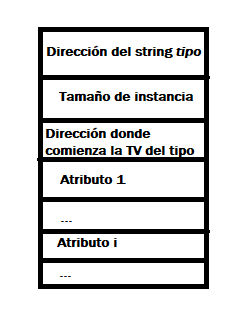
\includegraphics[scale=0.7]{Instancia.png}

\subparagraph{Paso de argumentos:}
	 En el paso de argumentos utilizamos la pila, liberando la memoria utilizada al terminar la ejecución de la función. 
\subparagraph{Creación de una instancia:}
	Para la creación de una instancia reservamos memoria utilizando \lstinline|sbrk|. Cada una de las instancias tendrá como atributos especiales su tipo y su tamaño, en la primera y última posición respectivamente; por tanto, al reservar memoria tenemos que hacerlo con un tamaño igual a la cantidad de atributos más dos.

\subparagraph{Localización de variables:}
	Para la localización de variables utilizamos la pila, y el acceso a cada una se controla a partir de un \textit{offset} que las representa dentro de \lstinline|$fp| para cada función. Este control se realiza a través de un diccionario en tiempo de compilación. 
	
\subsubsection{Llamado a función}

\subparagraph{Tabla Virtual:}
Al inicio de la ejecución del programa se construye una Tabla Virtual de la siguiente forma:

\begin{enumerate}
	\item Se reserva un espacio para cada tipo en la sección \textit{data}. 
	\item Se guarda, para la función X, la dirección de la etiqueta de la función Y adecuada, definida desde la generación de código intermedio. El \textit{offset} respecto al inicio de la tabla virtual se prefija en compilación de manera tal que si \textit{A} implementa \textit{X} y \textit{B} lo redefine, entonces \textit{X} se encuentra en el mismo \textit{offset} en ambas \textit{Tablas Virtuales}.
\end{enumerate}

\subparagraph{Decisión de la función a llamar:}
Para decidir qué función se debe llamar, basta localizar el \textit{offset} predefinido en compilación de la función, a partir de la dirección de \textit{Tabla Virtual} del tipo de la instancia, guardada como atriubuto en ésta.


\subparagraph{Pasos del llamado a función:}
		\begin{enumerate}
			\item Se salvan los registros utilizados: \lstinline|$fp, $ra|. (son los únicos que trascienden un llamado de función).
			\item Se pasan los argumentos a la pila.
			\item Se realiza la instrucción \lstinline|Jal function_name|, que guarda la dirección de retorno en el registro \lstinline|$ra|.
			\item Se sacan los argumentos de la pila. 
			\item Se restauran los registros. 
			\item Se toma el valor de retorno de \lstinline|$v0|. 
		\end{enumerate}
	La función llamada debe:
		\begin{enumerate}
			\item Mover \lstinline|$fp| a donde se encuentra \lstinline|$sp|. 
			\item Tomar sus argumentos de la pila. 
			\item Reservar memoria para todas sus variables locales. 
			\item Realizar las instrucciones que le correponden. 
			\item Liberar el espacio de la pila correspondiente a todas las variables locales. 
			\item Realizar un salto al contenido del registro \lstinline|$ra|. 
		\end{enumerate}


\subsubsection{Orden de herencia en MIPS para instrucción \lstinline|case|}
La relación de herencia se determina a través de unos atributos llamados \lstinline|order| y \lstinline|min_order|, creado desde la generación de código intermedio como atributo especial. Si A hereda de B, entonces seguramente \lstinline|min_order(B)<min_order(A)<order(A)<min_order(B)|. 

De esta forma garantizamos que en la ejecución de una instrucción \textit{case}, podamos decidirnos por la primera rama cuyo intervalo definido por \lstinline|(min_order(x), order(x))| esté contenido en en el mismo intervalo para el tipo de la expresión. Para garantizar que la primera sea la correcta, las ramas del \textit{case} se ordenan en tiempo de compilación por niveles de herencia.  

\subsubsection{Constructor de instancia en MIPS}

Para cada uno de los tipos, definimos una función especial llamada \lstinline|__init__|, que se crea en la fase de generación de código intermedio y se encarga de manejar la inicialización de los atributos heredados y los propios. 

\subsubsection{Manejo de \textit{strings} en memoria}

\begin{itemize}
	\item Un \textit{string} constante se reserva en la sección data en el inicio del programa, la estructura data que contiene los \textit{strings} esta construida desde la fase de generación de código intermedio.
	\item El espacio para guardar un \textit{string} que introduce el usuario se reserva utilizando el \lstinline|syscall| definido por \lstinline|sbrk| con un tamaño de \textit{buffer} de \textit{1024 bytes}. 
	\item El espacio para un \textit{string} resultante de una operación de cadena se reserva con el \lstinline|syscall| definido por \lstinline|sbrk| con el tamaño exacto necesario, que se conoce en ejecución a través de los argumentos del llamado.  
\end{itemize}

\subsubsection{Determinación del tipo en ejecución}

Dentro de cada instancia, como representamos anteriormente, se guarda un atributo especial que consiste en la dirección en memoria de la tabla virtual del tipo de ésta. Para acceder a esta dirección construimos una instrucción apropiada desde la fase de código intermedio, que se traduce en MIPS al acceso directo a la dirección en memoria predefinida donde sabemos que se encuentra este atributo. 

\label{end}

\end{document}

%===================================================================================

